\documentclass[aspectratio=169]{beamer}

\usetheme{Bruno}

\usepackage[T1]{fontenc}
\usepackage[utf8]{inputenc}
\usepackage[brazil]{babel}
\usepackage{graphicx}
\usepackage{booktabs}
\usepackage{lmodern}
\usepackage{microtype}
\usepackage{hyperref}
\usepackage{tikz}
\usepackage{xcolor}

\graphicspath{{fig/}}

% --- DUAS LOGOS ---
\IfFileExists{fig/logo2.png}{%
  \setbeamertemplate{headline}{%
    \vspace{2mm}
    \begin{beamercolorbox}[wd=\paperwidth, ht=1cm, dp=0.2cm]{}
      \hspace{3mm}
      \raisebox{4mm}{\includegraphics[height=0.4cm]{logo2.png}}
      \hfill
      \includegraphics[height=0.8cm]{logo1.jpeg}
      \hspace{3mm}
    \end{beamercolorbox}
  }
}{%
  \setbeamertemplate{headline}{}%
}

% METADADOS
\title{Detecção de Malha Viária em\\Imagens de Satélite}
\subtitle{Uma Abordagem Evolutiva com Visão Computacional Clássica}
\author{Beatriz Vocurca Frade \and Johnatan Augusto M. do Carmo \and Marina Alves Resende}
\institute{Universidade Federal de Minas Gerais\\Reconhecimento de Padrões -- PPGEE}
\date{Junho de 2026}

\begin{document}

% ============================================================
% CAPA
% ============================================================
\maketitle

% ============================================================
% SUMARIO
% ============================================================
\begin{frame}{Roteiro}
\tableofcontents
\end{frame}

% ============================================================
\section{Motivação e Problema}
% ============================================================

\begin{frame}{Motivação}
\begin{columns}
\column{0.6\textwidth}
\begin{itemize}
  \item Malha viária é infraestrutura crítica: planejamento urbano, logística, resposta a desastres.
  \item Mapeamento manual é \textbf{lento} e \textbf{custoso}.
  \item Imagens de satélite disponíveis em larga escala (Google Maps, Sentinel, etc.).
  \item Meta: extrair vias \textit{automaticamente} a partir de pixels, sem anotação humana.
\end{itemize}
\column{0.38\textwidth}
  % Substitua por imagem real quando disponível
  \fbox{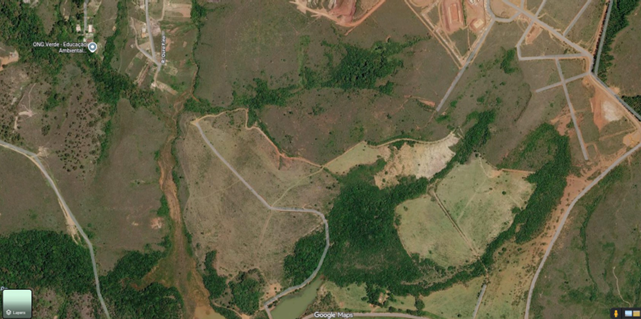
\includegraphics[width=\linewidth, height=4cm, keepaspectratio]{original.png}}
  \\\centering\small{Imagem de satélite de entrada}
\end{columns}
\end{frame}

\begin{frame}{Definição do Problema}
\begin{block}{Entrada}
  Imagem RGB de satélite (alta resolução, sem anotações).
\end{block}
\begin{block}{Saída esperada}
  \begin{itemize}
    \item \textbf{Máscara binária}: branco = via, preto = não-via
    \item \textbf{Sobreposição} da máscara na imagem original
    \item \textbf{Esqueleto} das vias (linhas de 1 pixel)
    \item \textbf{Grafo} da malha viária (nós = interseções/extremidades, arestas = trechos)
  \end{itemize}
\end{block}
\begin{alertblock}{Desafio central}
  Vias de terra, asfalto e concreto têm \textbf{aparência visual muito similar} ao solo exposto, telhados e campos agrícolas.
\end{alertblock}
\end{frame}

\begin{frame}{Pipeline Geral (comum às três versões)}
\centering
\begin{tikzpicture}[
  box/.style={draw, rounded corners, fill=blue!10, text width=2.2cm, align=center, minimum height=0.8cm, font=\small},
  arr/.style={->, thick}
]
  \node[box] (pre)  at (0,0)    {Pré-\\processamento};
  \node[box] (det)  at (3,0)    {Detecção\\de vias};
  \node[box] (pos)  at (6,0)    {Pós-\\processamento};
  \node[box] (skel) at (9,0)    {Esquele-\\tização};
  \node[box] (graf) at (12,0)   {Extração\\de grafo};
  \draw[arr] (pre)  -- (det);
  \draw[arr] (det)  -- (pos);
  \draw[arr] (pos)  -- (skel);
  \draw[arr] (skel) -- (graf);
\end{tikzpicture}

\bigskip
\begin{columns}
\column{0.19\linewidth}\centering\small Redimensionamento \\ Bilateral filter \\ CLAHE
\column{0.19\linewidth}\centering\small \textcolor{red}{\textbf{$\leftarrow$ foco das iterações}}
\column{0.19\linewidth}\centering\small Morfologia \\ Filtro de forma
\column{0.19\linewidth}\centering\small Zhang-Suen
\column{0.19\linewidth}\centering\small NetworkX \\ Grau de pixel
\end{columns}
\end{frame}

% ============================================================
\section{Versão 1 -- Segmentação por Cor}
% ============================================================

\begin{frame}{Versão 1 -- Abordagem Inicial por Cor}
\begin{columns}
\column{0.55\textwidth}
\textbf{Ideia central:} vias têm cor característica (asfalto cinza, terra quente). Segmentar por cor no espaço HSV/LAB.

\medskip
\begin{itemize}
  \item Classificação pixel a pixel em dois tipos de via:
  \begin{itemize}
    \item \textbf{Asfalto}: baixa saturação, tom cinzento
    \item \textbf{Terra}: matiz quente ($r > b$), saturação moderada
  \end{itemize}
  \item Limiares fixos no espaço HSV
  \item Pós-processamento morfológico simples (fechamento + abertura)
  \item Filtro de componentes por área e alongamento
\end{itemize}
\column{0.43\textwidth}
  % Adicione imagens da versão 1 aqui
  \fbox{\rule{0pt}{3.5cm}\hspace{\linewidth}} % placeholder
  \\\centering\small\textit{[Resultado da V1 -- adicionar imagem]}
\end{columns}
\end{frame}

\begin{frame}{Versão 1 -- Resultados e Limitações}
\begin{columns}
\column{0.48\textwidth}
\textbf{O que funcionou:}
\begin{itemize}
  \item Detectou vias de asfalto com bom contraste
  \item Simples e rápido de implementar
  \item Separou corretamente asfalto de vegetação em cenas urbanas
\end{itemize}

\medskip
\textit{[Completar com observações reais]}

\column{0.48\textwidth}
\textbf{Limitações identificadas:}
\begin{itemize}
  \item \textcolor{red}{Solo agrícola exposto = mesma cor de estrada de terra}
  \item \textcolor{red}{Campos extensos passavam no filtro de cor}
  \item Sem critério estrutural: não distingue ``via elongada'' de ``mancha de solo''
  \item Sensível à iluminação e ao horário da imagem
  \item Filtro de forma (alongamento do bounding box) facilmente enganado por campos retangulares
\end{itemize}
\end{columns}

\begin{alertblock}{Conclusão da V1}
  Cor sozinha é insuficiente. É necessário incorporar \textbf{informação estrutural}: vias são estreitas e elongadas.
\end{alertblock}
\end{frame}

% ============================================================
\section{Versão 2 -- Detecção Estrutural Multiescala}
% ============================================================

\begin{frame}{Versão 2 -- Motivação da Mudança}
\textbf{Hipótese reformulada:}

\begin{center}
\textit{``Uma via é uma estrutura \textbf{linear e estreita}. \\
Cor é apenas evidência secundária.''}
\end{center}

\bigskip
\textbf{Estratégia: 3 evidências independentes combinadas}

\medskip
\begin{columns}
\column{0.3\textwidth}
\centering
\textcolor{blue}{\textbf{Cue 1}}\\
Filtro de Frangi\\
\small(Hessiana multi-escala)
\column{0.3\textwidth}
\centering
\textcolor{blue}{\textbf{Cue 2}}\\
Top-hat Direcional\\
\small(morfológico, 6 ângulos)
\column{0.3\textwidth}
\centering
\textcolor{blue}{\textbf{Cue 3}}\\
Score de Cor Suave\\
\small(função contínua [0,1])
\end{columns}

\bigskip
\centering
$\text{prob} = 0{,}65 \times \max(\text{Frangi},\, \text{TopHat}) + 0{,}35 \times \text{Cor}$
\end{frame}

\begin{frame}{Versão 2 -- Filtro de Frangi (Hessiana Multi-escala)}
\begin{columns}
\column{0.55\textwidth}
\begin{itemize}
  \item Para cada escala $\sigma \in \{2, 4, 7\}$ pixels:
  \begin{itemize}
    \item Suaviza com Gaussiana de desvio $\sigma$
    \item Calcula derivadas de segunda ordem: $I_{xx}$, $I_{yy}$, $I_{xy}$
    \item Obtém autovalores $\lambda_a$, $\lambda_b$ da Hessiana 2D
  \end{itemize}
  \item Em uma via: $|\lambda_a| \approx 0$, $|\lambda_b|$ grande
  \item Medida de \textit{vesselness}:
  \[
    v = e^{-R_b^2 / 2\beta^2} \cdot \left(1 - e^{-S^2/2c^2}\right)
  \]
  onde $R_b = \lambda_a/\lambda_b$ (anisotropia) e $S = \|\lambda\|$ (força)
  \item Resultado: mapa [0,1] de estruturas lineares estreitas
\end{itemize}
\column{0.43\textwidth}
  \fbox{\rule{0pt}{3.8cm}\hspace{\linewidth}} % placeholder
  \\\centering\small\textit{[Mapa Frangi -- adicionar imagem]}
\end{columns}
\end{frame}

\begin{frame}{Versão 2 -- Top-hat Direcional e Score de Cor}
\begin{columns}
\column{0.48\textwidth}
\textbf{Top-hat Morfológico Direcional}
\begin{itemize}
  \item Elemento estruturante: linha de 12--35 px
  \item 6 orientações: 0°, 30°, 60°, 90°, 120°, 150°
  \item Top-hat branco (abertura): cristas \textbf{claras}
  \item Top-hat preto (fechamento): cristas \textbf{escuras}
  \item Detecta tanto asfalto escuro quanto concreto claro
  \item Comprimento limitado a 35 px: não responde a bordas de campos extensos
\end{itemize}
\column{0.48\textwidth}
\textbf{Score de Cor Suave}
\begin{itemize}
  \item Três modelos de superfície de via:
  \begin{itemize}
    \item \textbf{Asfalto}: baixa saturação, cinzento, $V \in [35, 230]$
    \item \textbf{Terra/cascalho}: quente ($R>B$), saturação baixa
    \item \textbf{Concreto}: alto valor, baixa saturação
  \end{itemize}
  \item Penalidades suaves para vegetação, sombra profunda, água e solo agrícola saturado
  \item Resultado: score contínuo em vez de limiar binário
\end{itemize}
\end{columns}
\end{frame}

\begin{frame}{Versão 2 -- Pós-processamento com Transformada de Distância}
\begin{columns}
\column{0.55\textwidth}
\textbf{Novidade-chave da V2: filtro de largura}

\medskip
\begin{itemize}
  \item Morfologia: fechamento + abertura
  \item Para cada componente conectado:
  \begin{enumerate}
    \item Calcula \textbf{transformada de distância euclidiana} (\texttt{cv2.distanceTransform})
    \item Extrai o \textbf{máximo local} = meia-largura do ponto mais largo
    \item Descarta se $\text{max\_hw} > \text{threshold}$ ($\approx$ 14--18 px)
  \end{enumerate}
  \item Um campo agrícola tem max\_hw $\gg$ 20 px $\Rightarrow$ \textbf{descartado}
  \item Uma via tem max\_hw $\in [2, 14]$ px $\Rightarrow$ \textbf{mantida}
\end{itemize}
\column{0.43\textwidth}
  \fbox{\rule{0pt}{3.8cm}\hspace{\linewidth}} % placeholder
  \\\centering\small\textit{[Transformada de distância -- adicionar imagem]}
\end{columns}
\end{frame}

\begin{frame}{Versão 2 -- Extração de Esqueleto e Grafo}
\begin{columns}
\column{0.48\textwidth}
\textbf{Esqueletonização (Zhang-Suen)}
\begin{itemize}
  \item Erosão iterativa que preserva topologia
  \item Máscara binária $\rightarrow$ linhas de 1 pixel
  \item Implementado via \texttt{skimage.morphology.skeletonize}
\end{itemize}

\medskip
\textbf{Extração do Grafo}
\begin{itemize}
  \item Grau 8-conectado por pixel do esqueleto
  \item \textbf{Nós:} pixels com grau 1 (extremidade) ou $\geq 3$ (interseção)
  \item \textbf{Arestas:} rastreio de caminho entre nós com comprimento em pixels
  \item \texttt{build\_full\_graph}: mantém \textit{todas} as componentes conectadas (não só a maior)
\end{itemize}
\column{0.48\textwidth}
  \fbox{\includegraphics[width=\linewidth, height=4cm, keepaspectratio]{esqueleto.png}}
  \\\centering\small{Esqueleto extraído}

  \medskip
  \fbox{\includegraphics[width=\linewidth, height=4cm, keepaspectratio]{grafo.png}}
  \\\centering\small{Grafo da malha viária}
\end{columns}
\end{frame}

\begin{frame}{Versão 2 -- Resultados}
\begin{columns}
\column{0.32\linewidth}
  \fbox{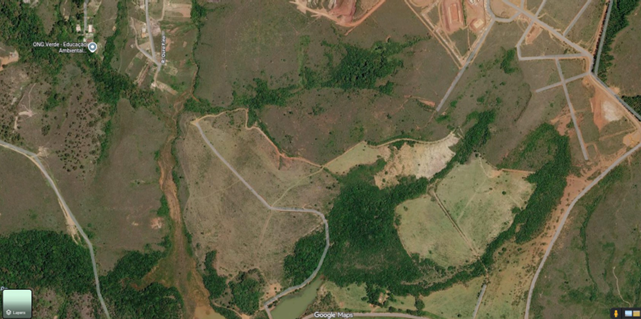
\includegraphics[width=\linewidth, height=3.5cm, keepaspectratio]{original.png}}
  \\\centering\small Original
\column{0.32\linewidth}
  \fbox{\includegraphics[width=\linewidth, height=3.5cm, keepaspectratio]{mascara.png}}
  \\\centering\small Máscara
\column{0.32\linewidth}
  \fbox{\includegraphics[width=\linewidth, height=3.5cm, keepaspectratio]{sobreposicao.png}}
  \\\centering\small Sobreposição
\end{columns}

\bigskip
\begin{columns}
\column{0.48\linewidth}
\textbf{Avanços em relação à V1:}
\begin{itemize}
  \item Filtro de largura (distância) elimina campos agrícolas
  \item Detecção estrutural não depende exclusivamente de cor
  \item Grafo preserva todas as rotas desconectadas
\end{itemize}
\column{0.48\linewidth}
\textbf{Limitações remanescentes:}
\begin{itemize}
  \item \textit{[Completar com observações reais da V2]}
  \item \textit{[Inserir métricas: \% de via, componentes, etc.]}
\end{itemize}
\end{columns}
\end{frame}

% ============================================================
\section{Versão 3 -- [Título a definir]}
% ============================================================

\begin{frame}{Versão 3 -- Evolução a Partir da V2}
\begin{center}
  \textit{[Slide a completar após implementação da V3]}
\end{center}

\medskip
\textbf{Motivação:} limitações identificadas na V2:
\begin{itemize}
  \item \textit{[Listar limitações que motivaram a V3]}
\end{itemize}

\medskip
\textbf{Mudanças na abordagem:}
\begin{itemize}
  \item \textit{[Descrever as novas técnicas]}
\end{itemize}
\end{frame}

\begin{frame}{Versão 3 -- Resultados}
\begin{center}
  \textit{[Slide a completar após implementação da V3]}
\end{center}

\medskip
\begin{columns}
\column{0.48\linewidth}
\textbf{Avanços em relação à V2:}
\begin{itemize}
  \item \textit{[Completar]}
\end{itemize}
\column{0.48\linewidth}
\textbf{Limitações remanescentes:}
\begin{itemize}
  \item \textit{[Completar]}
\end{itemize}
\end{columns}
\end{frame}

% ============================================================
\section{Análise Comparativa}
% ============================================================

\begin{frame}{Evolução das Versões -- Comparativo}
\centering
\begin{tabular}{lccc}
\toprule
\textbf{Característica} & \textbf{V1} & \textbf{V2} & \textbf{V3} \\
\midrule
Detector estrutural       & Não       & Frangi + Top-hat  & \textit{[a definir]} \\
Filtro de largura         & Não       & Dist. transform   & \textit{[a definir]} \\
Score de cor              & Limiar fixo & Suave [0,1]     & \textit{[a definir]} \\
Grafo completo (todos os segm.) & Não  & Sim              & \textit{[a definir]} \\
Falsos positivos (campos) & Alto      & Médio             & \textit{[a definir]} \\
Vias finas detectadas     & Parcial   & Sim ($\sigma=2$)  & \textit{[a definir]} \\
\bottomrule
\end{tabular}
\end{frame}

% ============================================================
\section{Conclusão}
% ============================================================

\begin{frame}{Lições Aprendidas}
\begin{columns}
\column{0.48\textwidth}
\textbf{Técnicas:}
\begin{enumerate}
  \item Cor sozinha não basta: solo agrícola e vias de terra são indistinguíveis por cor
  \item Informação estrutural (Frangi, top-hat) é essencial para separar vias de manchas
  \item Transformada de distância é um filtro geométrico eficaz: testa a largura \textbf{real} do componente
  \item Limiares adaptativos (percentil) generalizam melhor que valores fixos
\end{enumerate}
\column{0.48\textwidth}
\textbf{Processo:}
\begin{enumerate}
  \item Diagnóstico iterativo: cada versão parte dos erros da anterior
  \item Visualização interativa (máscara + sobreposição) acelera o ciclo de ajuste
  \item Grafo completo (todas as componentes) é mais informativo que apenas a maior componente
\end{enumerate}
\end{columns}
\end{frame}

\begin{frame}{Conclusão}
\begin{itemize}
  \item Desenvolvemos um pipeline de visão computacional \textbf{totalmente clássico} (sem redes neurais) capaz de extrair malha viária de imagens de satélite.
  \item A abordagem evoluiu em \textbf{três versões}, com diagnóstico explícito das limitações de cada uma.
  \item A combinação de \textbf{Frangi + top-hat direcional + score de cor} com filtro de largura por transformada de distância mostrou-se robusta para distinguir vias de campos agrícolas.
  \item O grafo extraído representa fielmente a conectividade da malha, preservando todos os segmentos detectados.
\end{itemize}

\bigskip
\centering
\textbf{Obrigado!}\\[4mm]
\small Beatriz Vocurca Frade \quad Johnatan Augusto M. do Carmo \quad Marina Alves Resende
\end{frame}

\end{document}
